% !TEX program = lualatex
\documentclass[12pt,a4paper]{ltjsarticle}
\usepackage{amsmath,amssymb,amsthm}
\usepackage{geometry}
\geometry{margin=2.5cm}
\usepackage{hyperref}
\hypersetup{colorlinks=true,linkcolor=blue,citecolor=blue,urlcolor=blue}
\usepackage{booktabs}
\usepackage{luatexja-fontspec}
\usepackage{graphicx}

\title{情報伝達の情報論的整理}
\author{木原 範昭（Noriaki Kihara）\\
WF System Co., Ltd.\\
大阪大学 基礎工学部 卒業}
\date{2026年4月\quad 研究ノート}

\begin{document}

\maketitle

\begin{abstract}
情報 $I$ に対して null 状態，等価判定，反転の3つの性質を定め，ディレイ回路 $F_D$ およびNOT演算回路の2種類の演算素子を定義する．これらの組み合わせにより，離散的な振動パターンおよび伝播パターンを構成し，それぞれの定式化が単振動，等速伝播，弦の基本振動の公式と数学的に同一の形をとることを示す．本稿は物理的主張を含まず，演算モデルとしての整合性のみを扱う．
\end{abstract}

\section{はじめに}

本稿は，情報の伝達を抽象的な演算処理として定式化し，その演算規則から導かれる離散的パターンを整理するものである．

具体的には，入力から出力への情報伝達を行うディレイ回路と，情報を反転するNOT演算回路の2つの演算素子を定義する．これらを単体で帰還接続した場合，直列に接続した場合，直列接続に帰還を加えた場合の3つの構成を考え，各構成から得られる式を既知の物理的公式と比較する．

\section{準備：定義と基本概念}

\subsection{本稿の範囲と限定}

本稿は以下を主張・証明するものでは\textbf{ない}：

\begin{itemize}
  \item \textbf{物理的実体に関する理論の証明}：本稿で扱うディレイ回路は情報演算上の抽象モデルであり，特定の物理系や物理法則の正当性を主張するものではない．
  \item \textbf{情報理論的な厳密性の証明}：本稿における「情報」はシャノン情報理論における情報量 $I$ とは異なり，情報理論の公理系に基づく厳密な議論を目的としない．
\end{itemize}

本稿が示すのは，入力から出力への情報伝達を抽象的な演算処理として定式化したとき，その\textbf{演算としての整合性}が保たれることである．

\subsection{ディレイ回路の定義}

\textbf{情報 $I$} とは，数値表現できるあらゆる情報を意味する．その形式はスカラー値，複素数値，行列，テンソルなど任意である．ただし，情報 $I$ は以下の性質を満たすものとする：

\begin{enumerate}
  \item \textbf{null 状態の存在}：情報が存在しない状態 $I = \mathrm{null}$ を定義できる．
  \item \textbf{null 判定の可能性}：任意の情報 $I$ に対して，$I = \mathrm{null}$ であるか否かを判定できる．$\mathrm{null}$ 同士の比較 $\mathrm{null} = \mathrm{null}$ は真とする．
  \item \textbf{クラスの定義}：情報はそれぞれクラス（型）に属する．任意の2つの情報 $I_a,\, I_b$ に対して，同一クラスに属するか否かを判定できる．例えば，実数と配列は異なるクラスである．$\mathrm{null}$ は任意のクラスに属するものとする（すなわち，任意の情報 $I$ に対して $\mathrm{null}$ と $I$ のクラス判定は常に同一クラスと判定される）．
  \item \textbf{等価判定の可能性}：同一クラスに属する任意の2つの情報 $I_a,\, I_b$ に対して，$I_a = I_b$（同一の情報であるか否か）を判定できる．
  \item \textbf{反転の定義}：任意の情報 $I$ に対して，その反転 $\overline{I}$ が定義できる．反転は同一クラス内の操作であり，$\overline{\overline{I}} = I$（二重反転で元に戻る）を満たすものとする．また，$\overline{\mathrm{null}} = \mathrm{null}$ とする．
\end{enumerate}

\textbf{情報伝達} とは，入力点 $\mathrm{IN}$ から出力点 $\mathrm{OUT}$ に情報 $I$ を伝達することと定める．

情報伝達を行う演算
\begin{equation}
\mathrm{OUT} = F_D(\mathrm{IN})
\end{equation}
における $F_D$ を\textbf{ディレイ回路}と定める．ディレイ回路は，入力情報と出力情報が同一クラスに属することを要求する．

\begin{figure}[htbp]
  \centering
  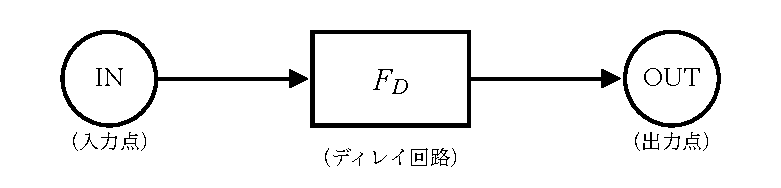
\includegraphics[width=0.5\textwidth]{fig1_delay_circuit.pdf}
  \caption{ディレイ回路}
  \label{fig:delay_circuit}
\end{figure}

\subsection{情報伝達における遅延の役割}

\begin{figure}[htbp]
  \centering
  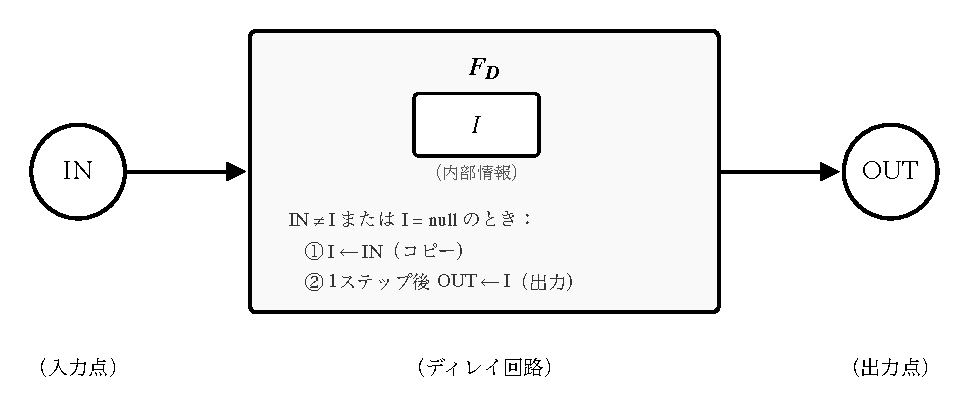
\includegraphics[width=0.7\textwidth]{fig2_delay_circuit_internal.pdf}
  \caption{ディレイ回路の内部構造}
  \label{fig:delay_circuit_internal}
\end{figure}

\paragraph{ディレイ回路の内部構造}

ディレイ回路 $F_D$ の内部から観測できる情報は以下の2つである：

\begin{itemize}
  \item \textbf{入力情報 $\mathrm{IN}$}：外部から与えられる情報．参照のみ可能であり，$F_D$ の内部から変更することはできない．
  \item \textbf{内部情報 $I$}：$F_D$ が内部に保持する情報．外部からは $\mathrm{OUT}$ として観測可能であるが，外部から変更することはできない．
\end{itemize}

\paragraph{初期状態}

ディレイ回路 $F_D$ の初期状態は $I = \mathrm{null}$，$\mathrm{OUT} = \mathrm{null}$ とする．

\paragraph{演算規則}

ディレイ回路 $F_D$ は以下の規則に従って動作する：

\begin{enumerate}
  \item $\mathrm{IN} \neq I$，または $I = \mathrm{null}$ の場合：
  \begin{itemize}
    \item 入力情報 $\mathrm{IN}$ を内部情報 $I$ にコピーする（$I \leftarrow \mathrm{IN}$）
    \item 1ステップの遅延の後，内部情報 $I$ を出力情報 $\mathrm{OUT}$ に出力する
  \end{itemize}
  \item $\mathrm{IN} = I$ の場合：
  \begin{itemize}
    \item 何もしない（$\mathrm{OUT}$ は変化しない）
  \end{itemize}
\end{enumerate}

\paragraph{外部からの観測可能量}

ディレイ回路 $F_D$ の演算は離散的なステップで進行する．外部から観測可能なのは，ディレイ演算が何回実行されたか（ディレイ回数 $n$）のみである．NOT演算回路の演算は遅延を伴わないため，ディレイ回数 $n$ には含めない．

\subsection{NOT演算回路}

NOT演算回路は，内部情報 $I$ を持ち，入力情報 $\mathrm{IN}$ を反転して遅延なし（即座）で出力する回路である．入力情報 $\mathrm{IN}$，内部情報 $I$，出力情報 $\mathrm{OUT}$ はすべて同一クラスに属するものとする．

\begin{itemize}
  \item \textbf{内部情報 $I$}：$\mathrm{IN}$ の反転を保持する．外部からは $\mathrm{OUT}$ として観測される．
\end{itemize}

\paragraph{演算規則}

\begin{enumerate}
  \item $\mathrm{IN} \neq \mathrm{null}$ の場合：
  \begin{itemize}
    \item $I \leftarrow \overline{\mathrm{IN}}$，$\mathrm{OUT} = I$
  \end{itemize}
  \item $\mathrm{IN} = \mathrm{null}$ かつ $I \neq \mathrm{null}$ の場合：
  \begin{itemize}
    \item $\mathrm{OUT} = I$（内部情報をそのまま出力する）
  \end{itemize}
  \item $\mathrm{IN} = \mathrm{null}$ かつ $I = \mathrm{null}$ の場合：
  \begin{itemize}
    \item $\mathrm{OUT} = \mathrm{null}$
  \end{itemize}
\end{enumerate}

\begin{figure}[htbp]
  \centering
  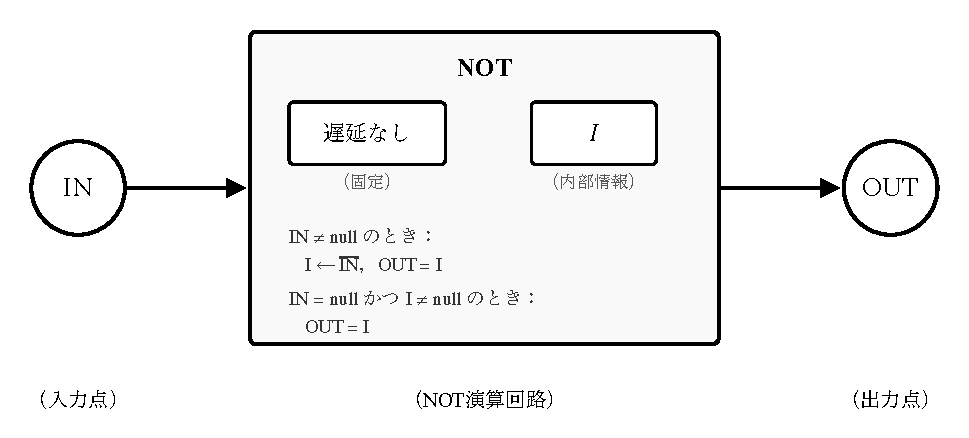
\includegraphics[width=0.5\textwidth]{fig3_not_circuit.pdf}
  \caption{NOT演算回路}
  \label{fig:not_circuit}
\end{figure}

\section{単振動回路}

ディレイ回路 $F_D$ とNOT演算回路を接続し，以下の帰還構造を構成する．$F_D$ の出力を NOT の入力に，NOT の出力を $F_D$ の入力に接続する．

\begin{figure}[htbp]
  \centering
  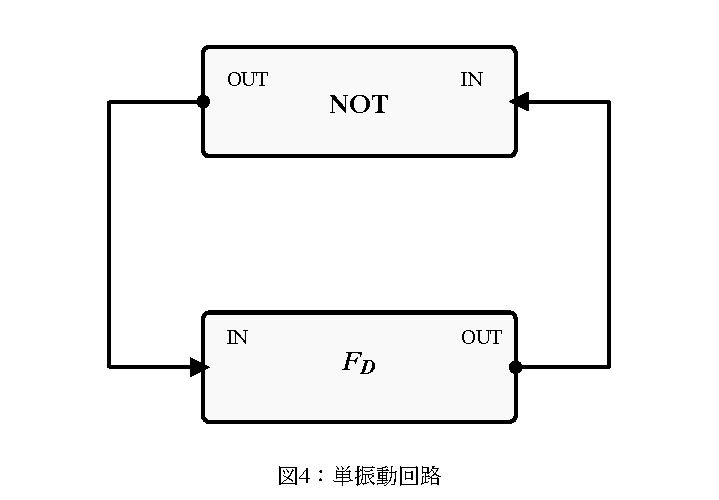
\includegraphics[width=0.6\textwidth]{fig4_oscillation_circuit.pdf}
  \caption{単振動回路}
  \label{fig:oscillation_circuit}
\end{figure}

\subsection{振動シーケンス}

単振動回路の各回における出力の遷移を以下に示す．

\begin{table}[htbp]
  \centering
  \begin{tabular}{ccc}
    \toprule
    ディレイ回数 $n$ & $F_D$ の OUT & NOT の OUT \\
    \midrule
    0 & $\mathrm{null}$ & $\mathrm{null}$ \\
    1 & $I$ & $\overline{I}$ \\
    2 & $\overline{I}$ & $I$ \\
    3 & $I$ & $\overline{I}$ \\
    4 & $\overline{I}$ & $I$ \\
    $\vdots$ & $\vdots$ & $\vdots$ \\
    \bottomrule
  \end{tabular}
\end{table}

$n \geq 1$ において，$F_D$ の出力は $I$ と $\overline{I}$ を交互に繰り返す．これは離散的な振動である．

\subsection{定式化}

情報 $I$ をスカラー値とし，反転を $\overline{I} = -I$ と定める．単振動回路の $F_D$ の出力は次のように表される：
\begin{equation}
x(n) = I \cdot (-1)^{n+1} \quad (n = 1, 2, 3, \ldots)
\end{equation}

すなわち，出力はディレイ回数 $n$ に対して $I$ と $-I$ を交互に繰り返す．

\section{開いた縄の情報伝達モデル}

$n$ 個のディレイ回路 $F_{D1}, F_{D2}, \ldots, F_{Dn}$ を直列に接続し，左端に入力点 $\mathrm{IN}_1$，右端に出力点 $\mathrm{OUT}_n$ を持つ構造を考える．これは自由端を持つ縄のモデルに相当する．

\begin{figure}[htbp]
  \centering
  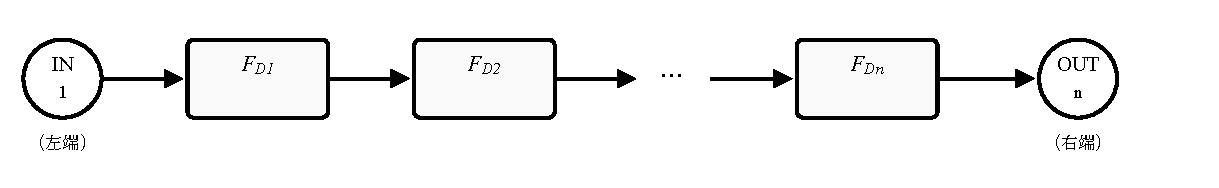
\includegraphics[width=0.85\textwidth]{fig5_open_string.pdf}
  \caption{開いた縄の情報伝達モデル}
  \label{fig:open_string}
\end{figure}

\subsection{伝播シーケンス}

ディレイ回数 $n = 0$ で $\mathrm{IN}_1$ に情報 $I$ を与えたときの各出力の遷移を示す．

\begin{table}[htbp]
  \centering
  \begin{tabular}{ccccccc}
    \toprule
    ディレイ回数 $n$ & $\mathrm{IN}_1$ & $\mathrm{OUT}_1$ & $\mathrm{OUT}_2$ & $\mathrm{OUT}_3$ & $\cdots$ & $\mathrm{OUT}_n$ \\
    \midrule
    0 & $I$ & $\mathrm{null}$ & $\mathrm{null}$ & $\mathrm{null}$ & $\cdots$ & $\mathrm{null}$ \\
    1 & $I$ & $I$ & $\mathrm{null}$ & $\mathrm{null}$ & $\cdots$ & $\mathrm{null}$ \\
    2 & $I$ & $I$ & $I$ & $\mathrm{null}$ & $\cdots$ & $\mathrm{null}$ \\
    3 & $I$ & $I$ & $I$ & $I$ & $\cdots$ & $\mathrm{null}$ \\
    $\vdots$ & $\vdots$ & $\vdots$ & $\vdots$ & $\vdots$ & $\ddots$ & $\vdots$ \\
    $n$ & $I$ & $I$ & $I$ & $I$ & $\cdots$ & $I$ \\
    \bottomrule
  \end{tabular}
\end{table}

情報 $I$ は，1回のディレイ演算ごとに隣接する $F_D$ へ1つずつ伝播する．

\subsection{定式化}

ディレイ回数 $n$ 後の情報の到達位置（先頭の $F_D$ の番号）を $k$ とすると：
\begin{equation}
k = n
\end{equation}

すなわち，情報の到達位置はディレイ回数に対して線形である．

\section{閉じた縄の情報伝達モデル}

第4章の開いた縄の構造において，$F_{Dn}$ の出力 $\mathrm{OUT}_n$ を NOT演算回路を介して $F_{D1}$ の入力 $\mathrm{IN}_1$ に接続し，負帰還ループを構成する．

\begin{figure}[htbp]
  \centering
  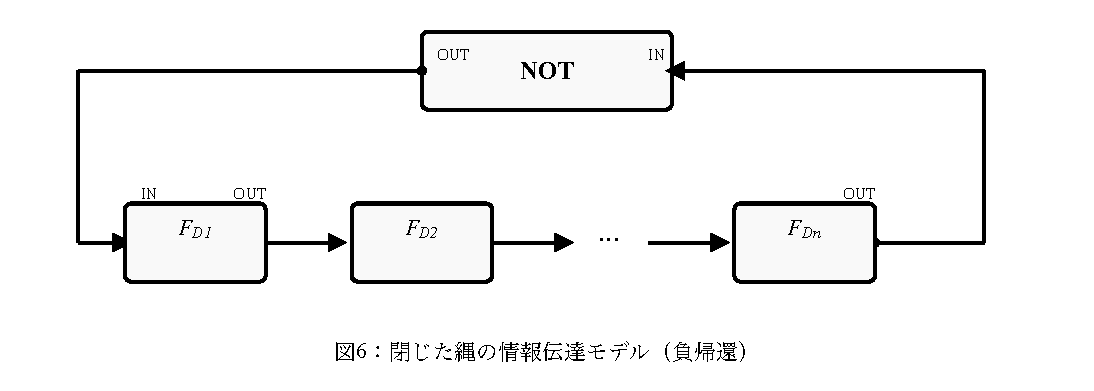
\includegraphics[width=0.85\textwidth]{fig6_closed_string.pdf}
  \caption{閉じた縄の情報伝達モデル（負帰還）}
  \label{fig:closed_string}
\end{figure}

\subsection{伝播シーケンス}

以下に $F_D$ を3個（$F_{D1}, F_{D2}, F_{D3}$）とした場合の伝播シーケンスを示す．初期条件として $F_{D1}$ に情報 $I$ を与える．

\begin{table}[htbp]
  \centering
  \begin{tabular}{ccccccl}
    \toprule
    ループ $m$ & ディレイ回数 $n$ & $\mathrm{IN}_1$ & $\mathrm{OUT}_1$ & $\mathrm{OUT}_2$ & $\mathrm{OUT}_3$ & NOT の OUT \\
    \midrule
    0 & 0 & $I$ & $\mathrm{null}$ & $\mathrm{null}$ & $\mathrm{null}$ & $\mathrm{null}$ \\
    0 & 1 & $I$ & $I$ & $\mathrm{null}$ & $\mathrm{null}$ & $\mathrm{null}$ \\
    0 & 2 & $I$ & $I$ & $I$ & $\mathrm{null}$ & $\mathrm{null}$ \\
    0 & 3 & $I$ & $I$ & $I$ & $I$ & $\overline{I}$ \\
    1 & 4 & $\overline{I}$ & $\overline{I}$ & $I$ & $I$ & $\overline{I}$ \\
    1 & 5 & $\overline{I}$ & $\overline{I}$ & $\overline{I}$ & $I$ & $\overline{I}$ \\
    1 & 6 & $\overline{I}$ & $\overline{I}$ & $\overline{I}$ & $\overline{I}$ & $I$ \\
    2 & 7 & $I$ & $I$ & $\overline{I}$ & $\overline{I}$ & $I$ \\
    2 & 8 & $I$ & $I$ & $I$ & $\overline{I}$ & $I$ \\
    2 & 9 & $I$ & $I$ & $I$ & $I$ & $\overline{I}$ \\
    3 & 10 & $\overline{I}$ & $\overline{I}$ & $I$ & $I$ & $\overline{I}$ \\
    3 & 11 & $\overline{I}$ & $\overline{I}$ & $\overline{I}$ & $I$ & $\overline{I}$ \\
    3 & 12 & $\overline{I}$ & $\overline{I}$ & $\overline{I}$ & $\overline{I}$ & $I$ \\
    \bottomrule
  \end{tabular}
\end{table}

各ループ $m$ ごとに，$I$ と $\overline{I}$ の波が $F_{D1}$ から $F_{Dn}$ へ伝播し，右端の NOT で反転されて次のループが始まる．1ループは $n$ 回の演算であり，$I$ と $\overline{I}$ の完全な1振動（2ループ）は $2n$ 回の演算である．

\subsection{定式化}

$n$ 個の $F_D$ からなる閉じた縄において，情報が全素子を通過するのに $n$ 回のディレイを要する．NOT での反転を含めた1振動（$I \to \overline{I} \to I$）は2ループであるから，1振動に要するディレイ回数は $2n$ 回である．
\begin{equation}
N_{\text{振動}} = 2n
\end{equation}

一方，両端が固定された弦の基本振動（モード1）では，波が弦の全長を1往復する間に1振動が完了する．弦を $n$ 個の離散要素に分割し，1要素の通過に1ステップを要するとすれば，1振動のステップ数は同じく $2n$ である．

両者の構造は同一である．

\section{考察}

本稿では，2種類の演算素子（ディレイ回路 $F_D$，NOT演算回路）と情報 $I$ の最小限の定義のみから，以下の3つの対応を得た．

\begin{table}[htbp]
  \centering
  \begin{tabular}{lll}
    \toprule
    構成 & 本モデルの結果 & 類似する物理的構造 \\
    \midrule
    $F_D$ + NOT（単体ループ） & $x(n) = I \cdot (-1)^{n+1}$ & 単振動 \\
    $F_D$ の直列接続（開いた縄） & 到達位置 $k = n$（線形伝播） & 等速伝播 \\
    $F_D$ 直列 + NOT（閉じた縄） & 1振動 $= 2n$ 回の演算 & 弦の基本振動（モード1） \\
    \bottomrule
  \end{tabular}
\end{table}

いずれの場合も，本モデルの演算規則から導かれるパターンは，類似する物理的構造と構造的な共通性を持つ．この共通性は，本モデルの演算的整合性の帰結であり，物理的主張を含むものではない．

\section{結論}

情報 $I$ に対して null 状態，等価判定，反転の3つの性質を定め，ディレイ回路 $F_D$ とNOT演算回路の2つの演算素子を定義した．これらの組み合わせにより，単振動，線形伝播，弦の基本振動に対応する離散的な振動・伝播パターンが構成され，それぞれが既知の物理的構造と同一のパターンを与えることを示した．

\begin{thebibliography}{9}
\bibitem{ref1} 原康夫『物理学基礎』学術図書出版社．
\bibitem{ref2} 戸田盛和『振動論』岩波書店．
\end{thebibliography}

\end{document}
